\documentclass{article}
\usepackage{graphicx}

\title{How DC circuits actually work}

\begin{document}
\maketitle

\section*{Introduction}
You probably know about circuits, maybe you even know how to solve for the current in a given branch in a circuit using Kirchoff's laws, but riddle me this - If a battery produces an electric field just like any other device, why are there no guidelines anywhere for how a circuit should be shaped?

\begin{center}
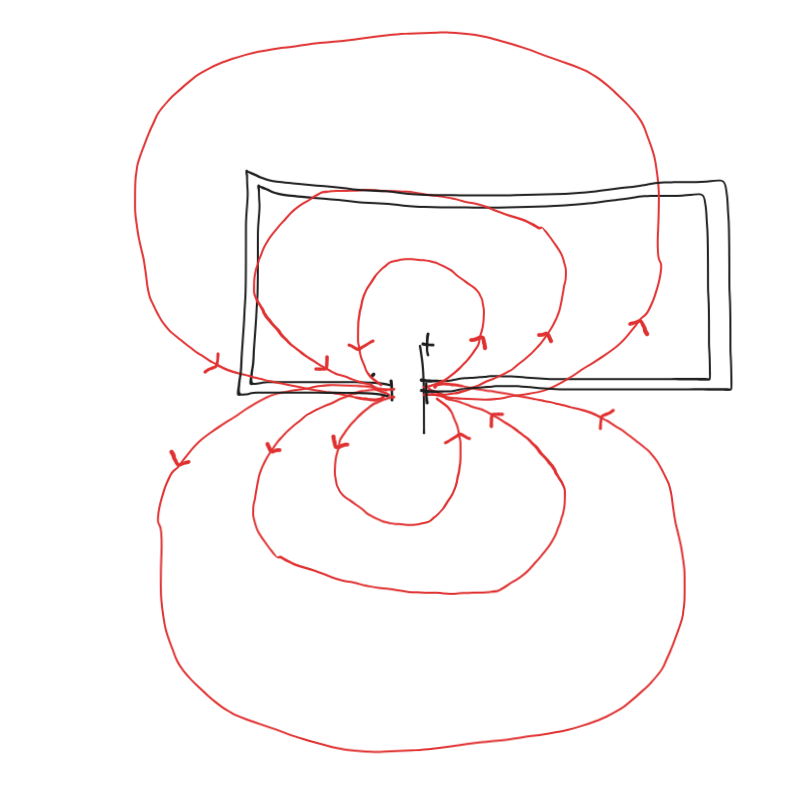
\includegraphics[scale=0.3]{1.png}    
\end{center}

Why is it that $V=I\cdot R$ applies for the entire circuit? If the electric field is what propels the electrons, and the electrons can only move in the wire, surely their speeds change dramatically from one place to another, right? These are the questions you will have answers to by the end of this explanation.

\newpage

\section*{0 - Isolation}

At this point in time, the battery is not connected to the wires but is turned on (so it is producing an electric field, the interesting stuff just hasn't happened yet).

\section*{1 - Contact}

As soon as the wires are in contact with the battery, the electrons will surge out of the negative terminal and into the wire, then they will bump around a bunch with the cations in the material of the wire.

Now the wire also has electrons and they can leave the cations they are bonded to if, say another electron repels them too much and a nearby cation (other than the one they are bonded to) attracts it. Temperature also plays a role in conductivity (the higher the temperature the more vigorously the lattice atoms vibrate with and so the more violent any collisions with electrons, increasing the resistivity). There are also other factors like the impurity levels in your wire.

Main thing is, those electrons are zooming out of the negative terminal, moreover the positive terminal is pulling the electrons from the wire in.

\begin{center}
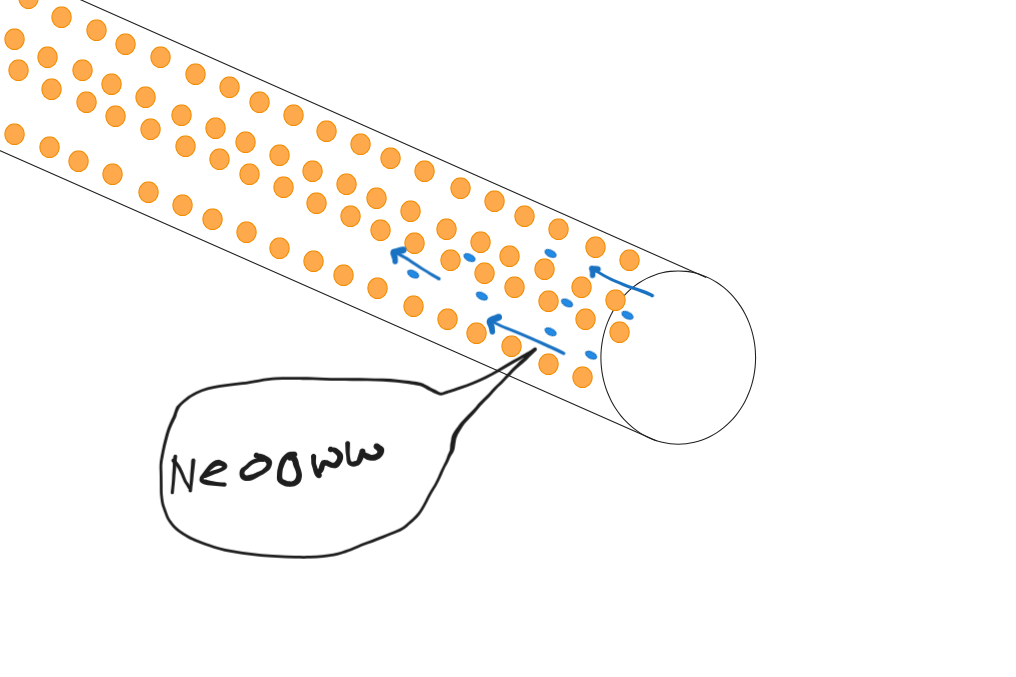
\includegraphics[scale=0.25]{2.png}    
\end{center}


\section*{2 - Combat}

Now the electrons have traveled down the wire and they're bouncing all about but now there's a problem, they're running into the walls of the wire way too often, there are two reasons for this.

Firstly, the electrons in the middle of the cross section are repelling them towards the perimeter of the wire.

Secondly, the wire is shaped in such a way that it follows some path to the negative terminal without going through the battery, this often leads to the electric field of the battery ramming the electrons into the boundaries.

Combine these two effects and enough electrons end up on the boundary to repel other electrons getting too close to the boundary and so they stay in line.

\end{document}
